\documentclass[a4paper,11pt]{ltjsarticle}

% --- パッケージの読み込み ---
\usepackage{amsmath, amssymb, amsthm, mathrsfs}
\usepackage{luatexja}
\usepackage{tikz}
\usetikzlibrary{cd, shapes, backgrounds, positioning, calc, arrows.meta, fit, patterns}
\usepackage{hyperref}
\usepackage{xcolor}
\usepackage{listings}
\usepackage{tcolorbox}
\usepackage{booktabs}

% --- ハイパーリンク設定 ---
\hypersetup{
    colorlinks=true,
    linkcolor=blue!70!black,
    citecolor=blue!70!black,
    urlcolor=blue!70!black
}

% --- 定理環境の定義 ---
\theoremstyle{definition}
\newtheorem{definition}{定義}[section]
\newtheorem{theorem}[definition]{定理}
\newtheorem{lemma}[definition]{補題}
\newtheorem{proposition}[definition]{命題}
\newtheorem{remark}[definition]{注釈}
\newtheorem{example}[definition]{例}

% --- マクロ定義 ---
\newcommand{\N}{\mathbb{N}}
\newcommand{\R}{\mathbb{R}}
\newcommand{\OmegaSpace}{\Omega}
\newcommand{\F}{\mathcal{F}}
\newcommand{\Prob}{\mathbb{P}}
\newcommand{\Expect}{\mathbb{E}}
\newcommand{\Tau}{\tau}
\newcommand{\Rank}{\rho}
\newcommand{\Tower}{\mathcal{T}}
\newcommand{\Layer}[1]{\mathrm{Layer}_{#1}}
\newcommand{\MinLayer}{\mathrm{minLayer}}
\newcommand{\Stopped}[2]{#1^{#2}} % Stopped process

% --- タイトル情報 ---
\title{\textbf{構造塔による確率論の再構築：Rank理論から任意停止定理へ} \\ \large --- Lean 4による形式化の数学的解説 ---}
\author{
    Lean Code Generation: \textbf{CODEX (OpenAI)} \\
    TeX Explanation \& Typesetting: \textbf{Gemini (Google)}
}
\date{\today}

\begin{document}

\maketitle

\begin{abstract}
本稿では、OpenAIのCODEXによって生成された一連のLean 4ファイルに基づき、確率論における停止時間とマルチンゲール理論を、より一般的な「ランク関数」と「構造塔 (Structure Tower)」の理論として再定式化する試みについて解説する。
具体的には、(1) ランク関数と構造塔の同型性、(2) 停止時間のランク関数としての解釈、(3) 停止過程の構造塔上の表現、(4) ランク理論に基づく有界任意停止定理 (Optional Stopping Theorem) の導出、の順に議論を展開する。
\end{abstract}

\tableofcontents

\newpage

% =========================================================================
% Section 1: Rank Tower
% =========================================================================
\section{ランク関数と構造塔の基礎理論}
\label{sec:rank_tower}
\textit{Based on: \texttt{RankTower.md}}

確率論への応用に入る前に、基礎となる抽象的な順序構造について定義する。ここでの目的は、要素に「階層（ランク）」を与えることと、空間を「層（Layer）」に分解することの数学的等価性を示すことである。

\subsection{ランク関数と構造塔の定義}

\begin{definition}[ランク関数]
集合 $X$ 上のランク関数とは、写像 $\Rank: X \to \N \cup \{\infty\}$ である。
本稿では主に、すべての要素が有限のランクを持つ場合（被覆性: $\forall x, \exists n, \Rank(x) \le n$）を扱う。
\end{definition}

\begin{definition}[構造塔 / Structure Tower]
集合 $X$ 上の構造塔 $\Tower$ とは、以下の性質を持つ部分集合の列 $(\Layer{n})_{n \in \N}$ である。
\begin{enumerate}
    \item \textbf{単調性}: $n \le m \implies \Layer{n} \subseteq \Layer{m}$
    \item \textbf{被覆性}: $X = \bigcup_{n \in \N} \Layer{n}$
\end{enumerate}
また、各要素 $x$ に対し、それが初めて現れる層のインデックスを $\MinLayer(x)$ と呼ぶ。
\end{definition}

\subsection{双方向の対応関係}
\texttt{RankTower.md} の核心は、この二つの概念が同型であるという定理である。

\begin{theorem}[正規形定理]
\begin{enumerate}
    \item ランク関数 $\Rank$ から、層 $\Layer{n} := \{x \mid \Rank(x) \le n\}$ を持つ構造塔を構成できる (\texttt{towerFromRank})。
    \item 構造塔 $\Tower$ から、ランク関数 $\Rank(x) := \min \{n \mid x \in \Layer{n}\}$ を構成できる (\texttt{rankFromTower})。
    \item この対応は互いに逆写像であり、数学的に同型である。
\end{enumerate}
\end{theorem}

\begin{figure}[h]
\centering
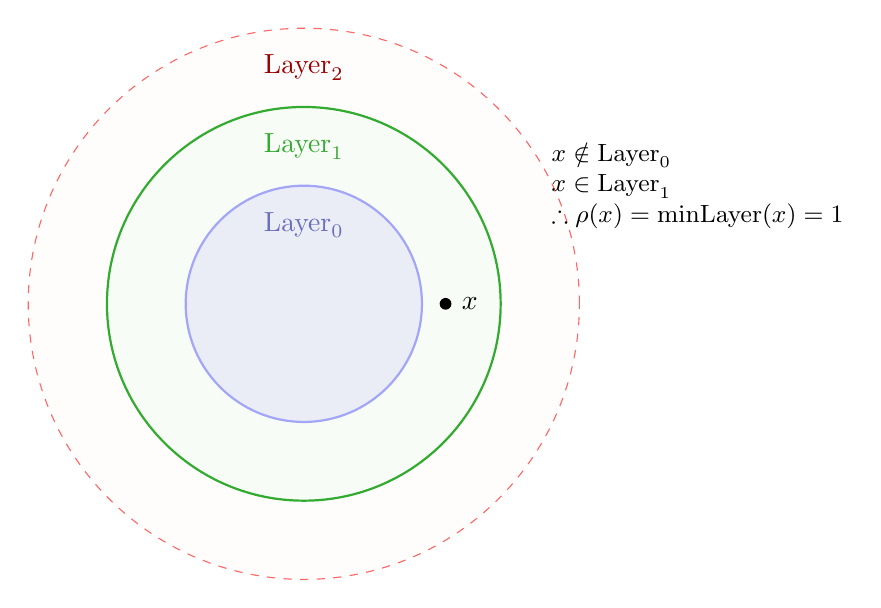
\begin{tikzpicture}[scale=1]
    % Layers as concentric circles
    \draw[fill=blue!10, draw=blue!60, thick] (0,0) circle (1.5cm);
    \node[blue!60!black] at (0, 1.0) {$\Layer{0}$};
    
    \draw[fill=green!10, draw=green!60!black, thick, fill opacity=0.3] (0,0) circle (2.5cm);
    \node[green!60!black] at (0, 2.0) {$\Layer{1}$};
    
    \draw[fill=red!5, draw=red!60, dashed, fill opacity=0.2] (0,0) circle (3.5cm);
    \node[red!60!black] at (0, 3.0) {$\Layer{2}$};

    % Element x
    \node[circle, fill, inner sep=1.5pt, label={right:$x$}] (x) at (1.8, 0) {};
    
    % Explanation
    \node[align=left, font=\small] at (5, 1.5) {
        $x \notin \Layer{0}$ \\
        $x \in \Layer{1}$ \\
        $\therefore \Rank(x) = \MinLayer(x) = 1$
    };
\end{tikzpicture}
\caption{構造塔とランク関数の視覚的解釈。要素 $x$ が初めて含まれる層の番号がそのランクとなる。}
\end{figure}

% =========================================================================
% Section 2: Stopping Time
% =========================================================================
\section{停止時間のランク理論的解釈}
\label{sec:stopping_time}
\textit{Based on: \texttt{StoppingTime\_C.md}}

前節の一般理論を確率論に適用する。ここでのキーアイデアは、\textbf{「停止時間とは、標本空間 $\OmegaSpace$ 上のランク関数である」}という視点の転換である。

\subsection{対応の辞書}

確率空間 $(\OmegaSpace, \F, \Prob)$ とフィルトレーション $(\F_n)$ を考える。

\begin{table}[h]
\centering
\caption{ランク理論と確率論の対応}
\begin{tabular}{lcl}
\toprule
\textbf{ランク理論} & $\longleftrightarrow$ & \textbf{確率論} \\ \midrule
集合 $X$ & $\longleftrightarrow$ & 標本空間 $\OmegaSpace$ \\
ランク関数 $\Rank$ & $\longleftrightarrow$ & 停止時間 $\Tau$ \\
層 $\Layer{n}$ & $\longleftrightarrow$ & 停止集合 $\{\Tau \le n\}$ \\
$\MinLayer(x)$ & $\longleftrightarrow$ & 初めて可測になる時刻 \\
\bottomrule
\end{tabular}
\end{table}

\subsection{停止集合と層の一致}
\texttt{StoppingTime\_C.md} では、停止時間 $\Tau$ をランク関数 $\Rank_\Tau(\omega) := \Tau(\omega)$ と見なし、そこから構造塔を誘導している。

\begin{theorem}[停止集合の層表現]
停止時間 $\Tau$ から誘導される構造塔の第 $n$ 層は、停止集合と一致する。
\[
    \Layer{n} = \{\omega \in \OmegaSpace \mid \Tau(\omega) \le n\}
\]
\end{theorem}
この定理 (\texttt{stoppingSet\_eq\_layer}) により、確率論における「事象の確定」というプロセスが、構造塔における「層の被覆」として幾何学的に理解される。

\begin{remark}
逆に、フィルトレーション自体も構造塔と見なせる。標本点 $\omega$ に対して、単集合 $\{\omega\}$ が初めて $\F_n$ で識別可能になる（可測集合として分離できる）時刻をランクと定義することで、フィルトレーションから停止時間を再構成することも可能である (\texttt{rankFromFiltrationTower})。
\end{remark}

% =========================================================================
% Section 3: Martingale Structure
% =========================================================================
\section{マルチンゲールとランク構造}
\label{sec:martingale}
\textit{Based on: \texttt{Martingale\_RankStructure.md}}

次に、この構造塔の上で定義される確率過程、特にマルチンゲールについて考察する。

\subsection{停止過程 (Stopped Process) のランク表現}
マルチンゲール $M = (M_n)$ を停止時間 $\Tau$ で止めた過程 $M^\Tau$ は、通常 $M^\Tau_n(\omega) = M_{\min(n, \Tau(\omega))}(\omega)$ と定義される。
これをランク理論の言葉で翻訳すると、以下のようになる。

\begin{definition}[ランク停止過程]
ランク関数 $\Rank$ (すなわち $\Tau$) に基づく停止過程 \texttt{rankStoppedProcess} は、層構造に従って値を「凍結」させる操作である。
\[
    \text{rankStoppedProcess}(M, \Rank, n, \omega) = M_{\min(n, \Rank(\omega))}(\omega)
\]
\end{definition}

\subsection{マルチンゲール性の保存}
このファイルは「薄いラッパー」として機能し、既存のマルチンゲール理論の定理をランク理論の語彙に翻訳している。

\begin{theorem}[有界ランクでのマルチンゲール性]
ランク関数 $\Rank$ が有界（$\exists K, \forall \omega, \Rank(\omega) \le K$）であり、対応する構造塔がフィルトレーションに適合しているならば、停止過程 $M^\Rank$ もまたマルチンゲールとなる。
\end{theorem}

\begin{figure}[h]
\centering
\begin{tikzpicture}[xscale=1.5, yscale=0.8]
    % Draw paths
    \draw[gray!50] (0,0) -- (1,1) -- (2,0) -- (3,1) -- (4,2);
    \draw[gray!50] (0,0) -- (1,-1) -- (2,-2) -- (3,-1) -- (4,0);
    
    % Stopping line (conceptual)
    \draw[blue, thick, dashed] (0,2.5) -- (4,2.5) node[right] {Rank Limit $K$};
    
    % Specific path stopping
    \draw[thick, ->] (0,0) -- (1,1) -- (2,2) node[above] {$\Rank(\omega)=2$} -- (3,2) -- (4,2);
    \node[right, font=\footnotesize] at (4,2) {Stopped Value};
    
    \node[align=left, font=\small] at (2, -3) {
        ランク（停止時刻）に達すると、\\
        その層の値が以降の全ての層に\\
        コピーされる（値の凍結）。
    };
\end{tikzpicture}
\caption{停止過程のイメージ。ランク $\Rank(\omega)$ に到達した時点で、プロセスは構造塔の「上層」へ向かって定数値として伝播する。}
\end{figure}

% =========================================================================
% Section 4: Optional Stopping Theorem
% =========================================================================
\section{ランク理論による任意停止定理 (OST)}
\label{sec:ost}
\textit{Based on: \texttt{2025-12-06\_OptionalStopping\_RankTheory.md}}

最後に、これまでの準備のもとで、確率論の重要な定理である任意停止定理 (Optional Stopping Theorem) をランク理論の枠組みで証明する。

\subsection{定理の主張}

\begin{theorem}[Bounded Optional Stopping - Rank版]
マルチンゲール $M$ と有界なランク関数（停止時間） $\Tau$ に対し、任意の層（時刻） $n$ において、停止過程の期待値は初期値の期待値と等しい。
\[
    \Expect[\text{rankStoppedProcess}(M, \Tau, n)] = \Expect[M_0]
\]
特に、十分大きな $n$ （ランクの上界 $K$ 以上）においては、停止時刻での値 $M_\Tau$ の期待値と一致する。
\[
    \Expect[M_\Tau] = \Expect[M_0]
\]
\end{theorem}

\subsection{証明の構造と意義}
Leanによる証明は以下のロジックに従っている。

\begin{enumerate}
    \item \textbf{有界性}: ランク関数が有界であるため、ある層 $K$ ですべての標本点が「停止済み」となる。
    \item \textbf{マルチンゲール性}: 前節の結果より、停止過程自体がマルチンゲールである。
    \item \textbf{期待値の保存}: マルチンゲールの定義より $\Expect[M^\Tau_n] = \Expect[M^\Tau_0] = \Expect[M_0]$。
    \item \textbf{普遍性}: この等式は構造塔のどの層 $n$ で評価しても成立する (\texttt{rankOST\_expectation\_constant})。
\end{enumerate}

この定式化の数学的・教育的意義は、OSTを「確率過程の収束」という解析的な問題から、\textbf{「構造塔上の不変量（マルチンゲール性）の保存」という代数的・構造的な問題}へと視点を移した点にある。

\section{結論}
一連のLeanファイルは、確率論における停止時間とOSTを、ランク理論というより抽象的な視点から再構築することに成功している。
\begin{itemize}
    \item \textbf{RankTower}: 順序構造の基礎付け。
    \item \textbf{StoppingTime}: 確率論的対象の構造的解釈。
    \item \textbf{Martingale}: 構造上のダイナミクス。
    \item \textbf{OptionalStopping}: 構造が保存する不変量。
\end{itemize}
このアプローチは、確率論を「計算」の学問から「構造」の学問へと昇華させるブルバキ的な精神を体現していると言える。

\end{document}